\chapter{\texorpdfstring{\tool[]}{SojiTantei}: A Tool To Aid In Library Migrations}
\label{sec:specification}

\begin{comment}
as well as showing the results for the exploratory study replication performed with the tool.
\end{comment}
Once the exploratory study was finished I had a better understanding of what were the features that will be useful in a tool to help the developers have a better insight of their projects and the relation with the third-party libraries. Among those features the most important one is the ability to trace third-party library function-calls since it will allow the user to understand if a vulnerable function in the library is been reached or not.

As mentioned before in Chapter \ref{sec:background}, I am working on the automation of the function-call extraction for challenge number 2, by using syntax analysis in the project code files. 

In this Chapter I will be explaining in detail the behavior of \tool[] but before that I will be explaining the origin of the name. \tool[] is a combination of two Japanese words. S\={o}ji (\begin{CJK}{UTF8}{min}掃除\end{CJK}) which means clean and Tantei (\begin{CJK}{UTF8}{min}探偵\end{CJK})
that means detective. The idea is that the tool will work as a \textit{detective}, allowing the developer to know the details of their projects regarding the relations with third-party libraries and based on those details help the developer to perform the corresponding \textit{cleaning} (i.e. update) for the project.

%Approach
%\section{Approach}
%%%%%%%%%%%%%%%%%%%%%%%%%%%%%%%%%%%%%
\begin{figure}[ht!]
\centering
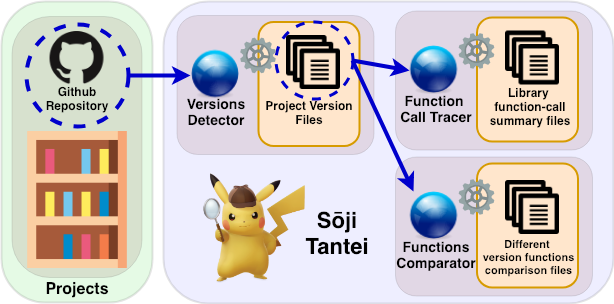
\includegraphics[width=1\textwidth]{images/tool_approach.png}
\caption{\tool[] Functionalities Diagram. (i) Versions Detector (ii) Function-Call Tracer (iii) Functions Comparator}
\label{fig:sojiApproach}
\end{figure}
%%%%%%%%%%%%%%%%%%%%%%%%%%%%%%%%%%%%%  

Figure \ref{fig:sojiApproach} gives an overview of the features of \tool[] which will be detailed further on.
Since the initial target for the tool is the \textit{nodeJS} ecosystem, the tool was programmed using \textit{JavaScript} and \textit{npm} libraries and it is divided in a series of scripts that can be run separately depending on the information required.
The goal of \tool[] is to analyze nodeJS projects, to achieve that goal it is necessary to download the git repository of the projects that will be analyzed since they will be the input for the first functionality. 
\enlargethispage{\baselineskip}
Once the git repository of the projects have been downloaded the user can proceed to use the following functions.\\

%First Functionality
\textbf{Versions Detector:}\\
It was mentioned before that both client projects and third-party libraries release new versions of their code from time to time. 
In order to be able to analyze a specific version of the library the first step is to detect all the available versions of the code.
To achieve this I used the npm library \textit{nodegit}\footnote{website at \url{https://www.nodegit.org/}}, which allows the usage of customized \textit{git} commands within a nodeJS project.
\\
For this functionality two methods to obtain the available versions were implemented:

\underline{a. Version in \textit{package.json}}:
The first approach is to get the latest commit available in the git repository and going backwards until the first commit is reached. 
For every commit the file \textit{package.json} is analyzed to get the version number as shown in Figure \ref{fig:pkgVerExample}. 

%%%%%%%%%%%%%%%%%%%%%%%%%%%%%%%%%%%%%
\begin{figure}[ht!]
\centering
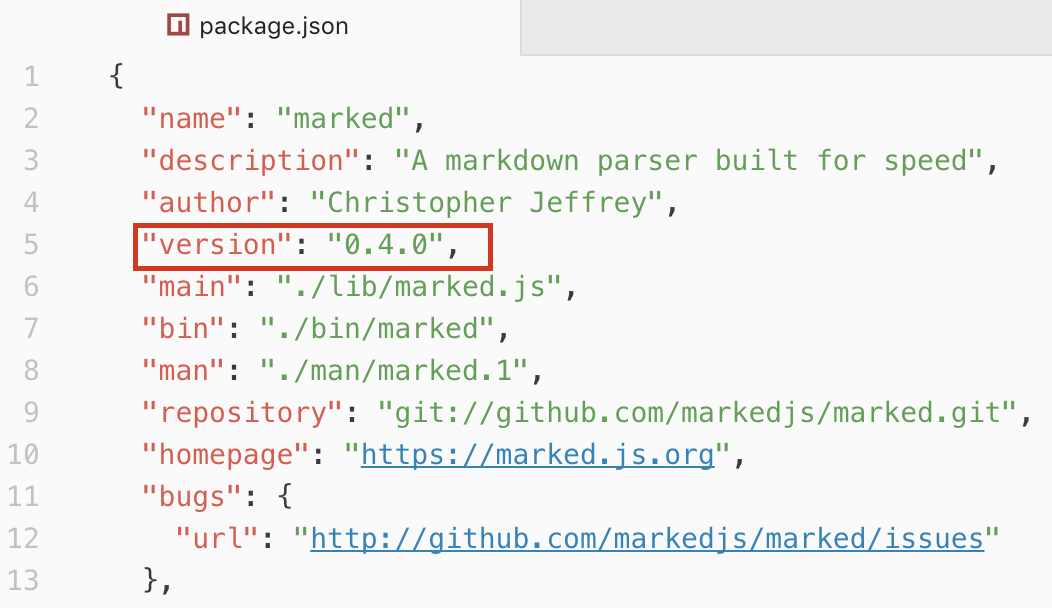
\includegraphics[width=1\textwidth]{images/ver_pkg_example.png}
\caption{Example of version information in \textit{package.json} file for \textit{marked} library}
\label{fig:pkgVerExample}
\end{figure}
%%%%%%%%%%%%%%%%%%%%%%%%%%%%%%%%%%%%%    

Once the version changes between 2 commits, the latest version number (i.e. the first appearance of that version in the commit history) is stored along with the hash id related to the commit for its usage in the next step. Figure \ref{fig:listExample} is showing an example of the list generated.

%%%%%%%%%%%%%%%%%%%%%%%%%%%%%%%%%%%%%
\begin{figure}[ht!]
\centering
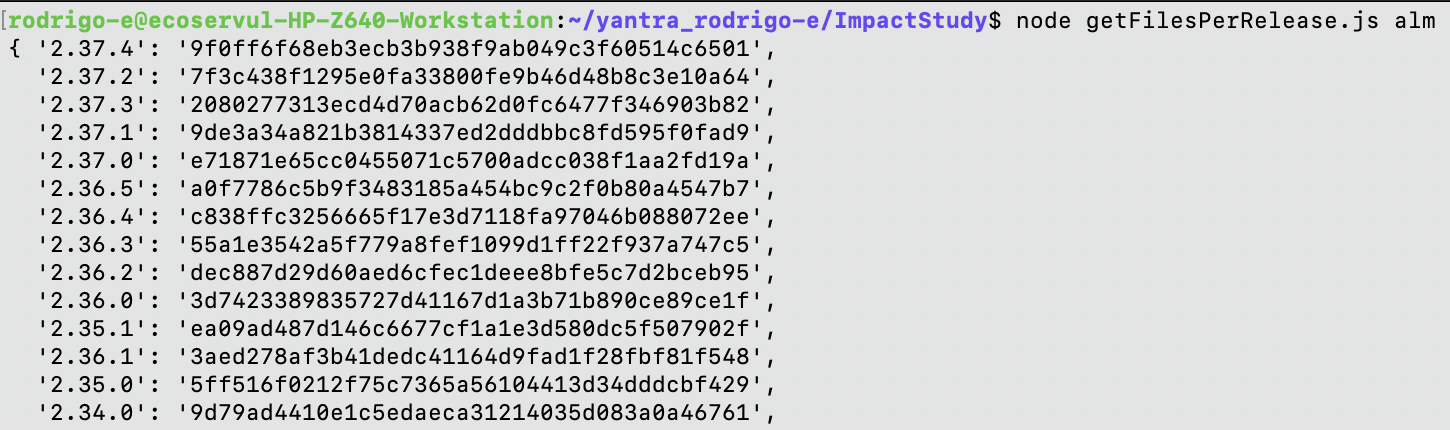
\includegraphics[width=1\textwidth]{images/list_example.png}
\caption{Example of the list created containing the version number and the hast id for the \textit{alm} project}
\label{fig:listExample}
\end{figure}
%%%%%%%%%%%%%%%%%%%%%%%%%%%%%%%%%%%%% 

When the list of versions and hash ids has been completed, as shown in the Figure \ref{fig:fileListExample} the tool proceeds to create a file named R\_\{version\}.txt containing the list of the files with extension \textit{js} or \textit{jsx} that exists in each of the hash id commits.

%%%%%%%%%%%%%%%%%%%%%%%%%%%%%%%%%%%%%
\begin{figure}[ht!]
\centering
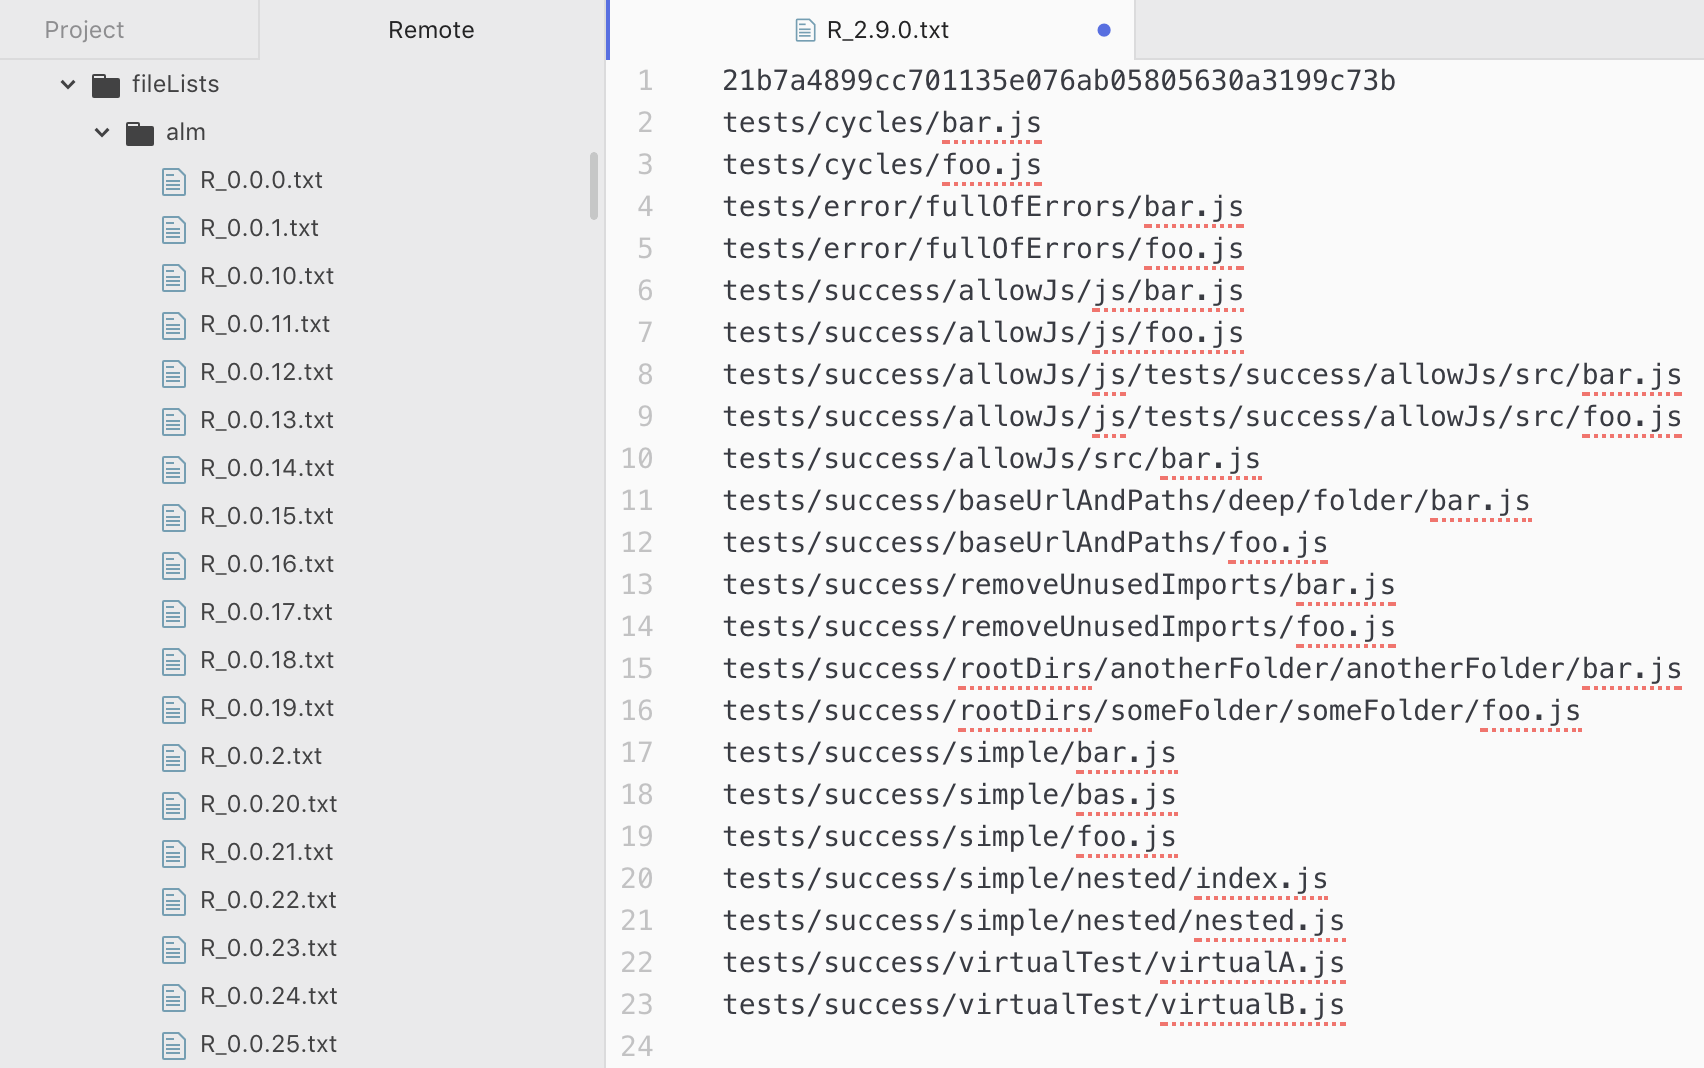
\includegraphics[width=1\textwidth]{images/file_list_example.png}
\caption{Example of the output generated by \tool[] after getting version release numbers for the \textit{alm} project}
\label{fig:fileListExample}
\end{figure}
%%%%%%%%%%%%%%%%%%%%%%%%%%%%%%%%%%%%% 

To follow this approach the user needs to run the script called "\textit{getFilesPerRelease.js}" inputting in the first and only parameter the name of the project to be analyzed. \\

\underline{b. Version in commit tag}:
The second approach implemented to get the different release versions available in a project is by getting the release tags along with the hash id in the commit history of the git repository as shown in Figure \ref{fig:tagExample}.

Just like the previous approach, with the information obtained, the tool creates a file named R\_\{version\}.txt containing the list of the files with extension \textit{js} or \textit{jsx} that exists in each of the tags retrieved. 
This will generate the same output as shown in Figure \ref{fig:fileListExample} previously.

To follow this approach the user needs to run the script called "\textit{getTags.js}" inputting in the first and only parameter the name of the project to be analyzed. 

%%%%%%%%%%%%%%%%%%%%%%%%%%%%%%%%%%%%%
\begin{figure}[ht!]
\centering
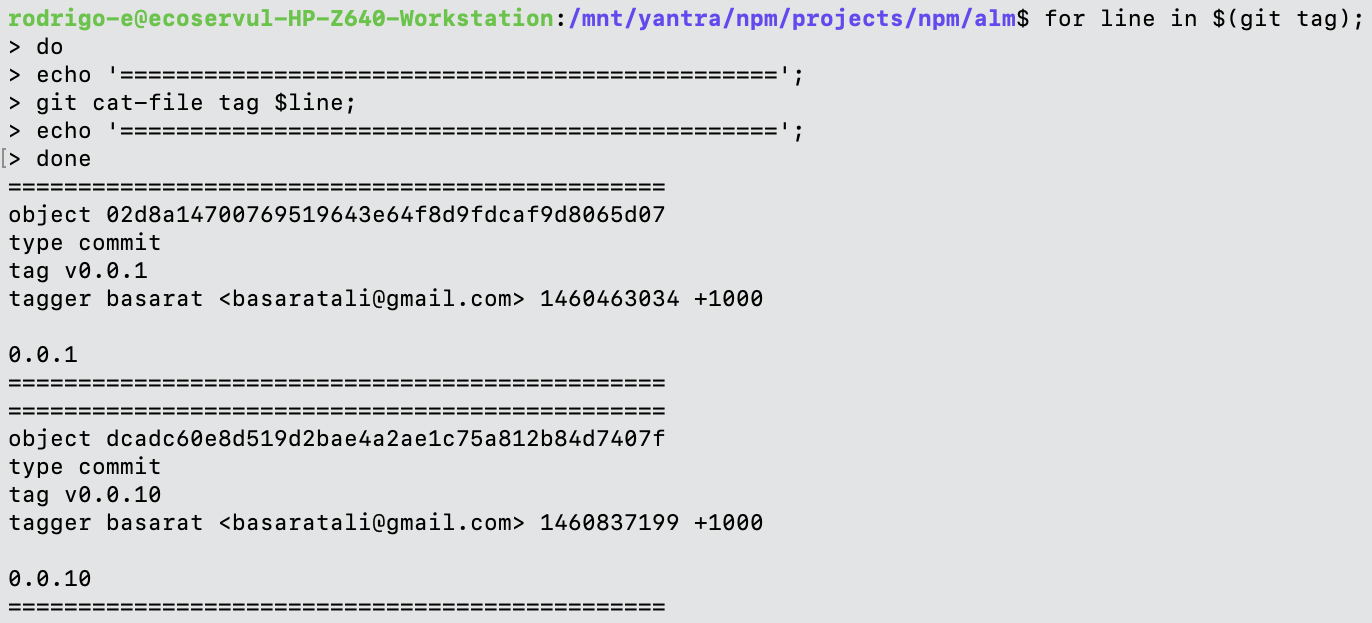
\includegraphics[width=1\textwidth]{images/tag_example2.png}
\caption{Example of the tags saved in the git commits for the \textit{alm} project}
\label{fig:tagExample}
\end{figure}
%%%%%%%%%%%%%%%%%%%%%%%%%%%%%%%%%%%%% 

The output generated in this functionality will be used in the next functions of the tool. For both of the approaches used, the tool depends on the developer including the version either in the \textit{package.json} file or in a tag when creating a release commit. Fortunately most of the users include the version in the \textit{package.json} file.\\

%Second Functionality
\textbf{Function-Call Tracer:}\\
For this functionality the tool uses the library \textit{esprima}\footnote{website at \url{http://esprima.org/}} to perform a syntax analysis of every \textit{js} or \textit{jsx} file on a project provided by the output of Versions Detector. 
%\enlargethispage{\baselineskip}
When performing the syntax analysis of a file, the tool will search all the \textit{require} statements to get the libraries that are been used in the file and the methods called for those libraries. This is achieved by doing a recursive tokenization because the \textit{require} statement is first stored in a local variable and then the methods of the library are invoked through that local variable, this makes the analysis of function-calls a hard to perform task. Figure \ref{fig:libExamples} shows an example of how the function calls could be performed in the nodeJS ecosystem and what will be the output of the functionality. 

I mentioned before in Chapter \ref{sec:background} that there are many ways to perform a function call in JavaScript, for this functionality I will be focusing on \textit{function expression} type which is the most common type of call\footnote{For more information please consult the follwing url: \url{https://dmitripavlutin.com/6-ways-to-declare-javascript-functions/\#2functionexpression}} for third-party libraries. 

%%%%%%%%%%%%%%%%%%%%%%%%%%%%%%%%%%%%%
\begin{figure}[ht!]
\centering
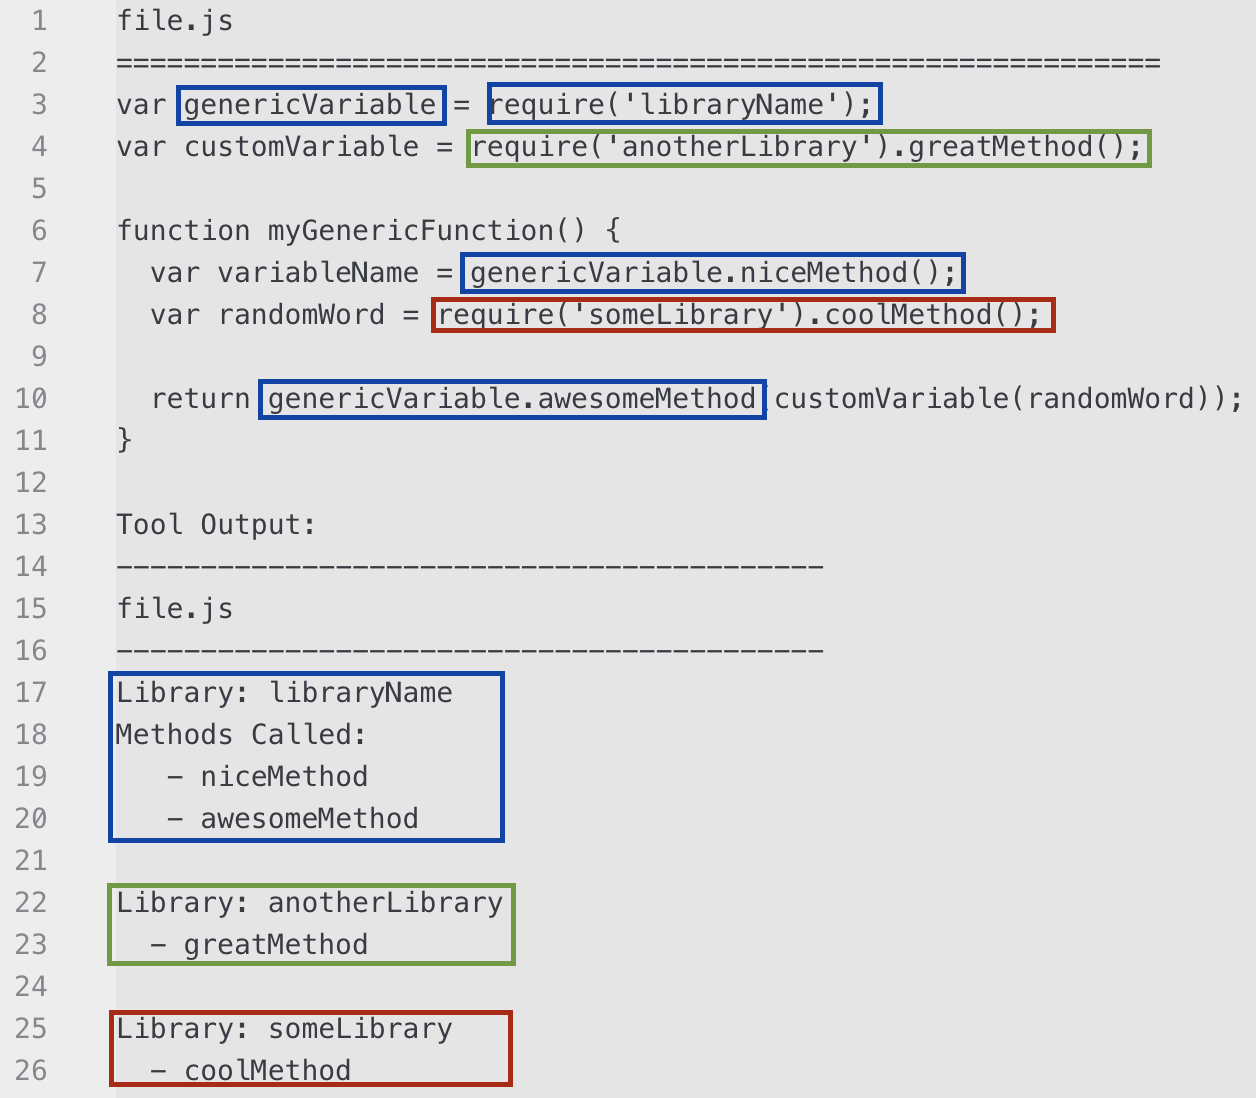
\includegraphics[width=1\textwidth]{images/libraries_example.png}
\caption{Example of the different method calls for the nodeJS ecosystem}
\label{fig:libExamples}
\end{figure}
%%%%%%%%%%%%%%%%%%%%%%%%%%%%%%%%%%%%% 

Since nodeJS programs are not compiled as those in Java, there is no easy way to get the function calls of the program since we cannot use a dynamic approach. Therefore, a syntactic analysis seemed like the best approach to be used in this case.

To execute this functionality the user needs to execute the script called \textit{syntaxChecker.js} and input the name of the project to be analyzed in the first parameter. 
There are two possible executions of the script, 
(i) running the script without extra parameters will get the function-calls for all the versions of the project included in the output of Versions Detector. 
(ii) running the script inputting from the second parameter the names of version files (i.e. R\_\{version\}.txt) included in the output of Versions Detector will perform the analysis on those files only.

The output of this functionality is a single file containing a list of the third-party library function-calls per file (as shown previously in Figure \ref{fig:listExample}) and a generalized list of all the function-calls in the project.\\

%Third Functionality
\textbf{Functions Comparator:}\\
The final function of \tool[] makes use of the libraries \textit{function-extractor}\footnote{website at \url{https://www.npmjs.com/package/function-extractor}} and \textit{deep-diff}\footnote{website at \url{https://www.npmjs.com/package/deep-diff}} and allows the user to get a comparison of the functions of two different versions of the project to get information about (i) functions added, (ii) functions deleted and (iii) functions edited. Figure \ref{fig:compExample} shows an example of the output generated by this functionality.

%%%%%%%%%%%%%%%%%%%%%%%%%%%%%%%%%%%%%
\begin{figure}[ht!]
\centering
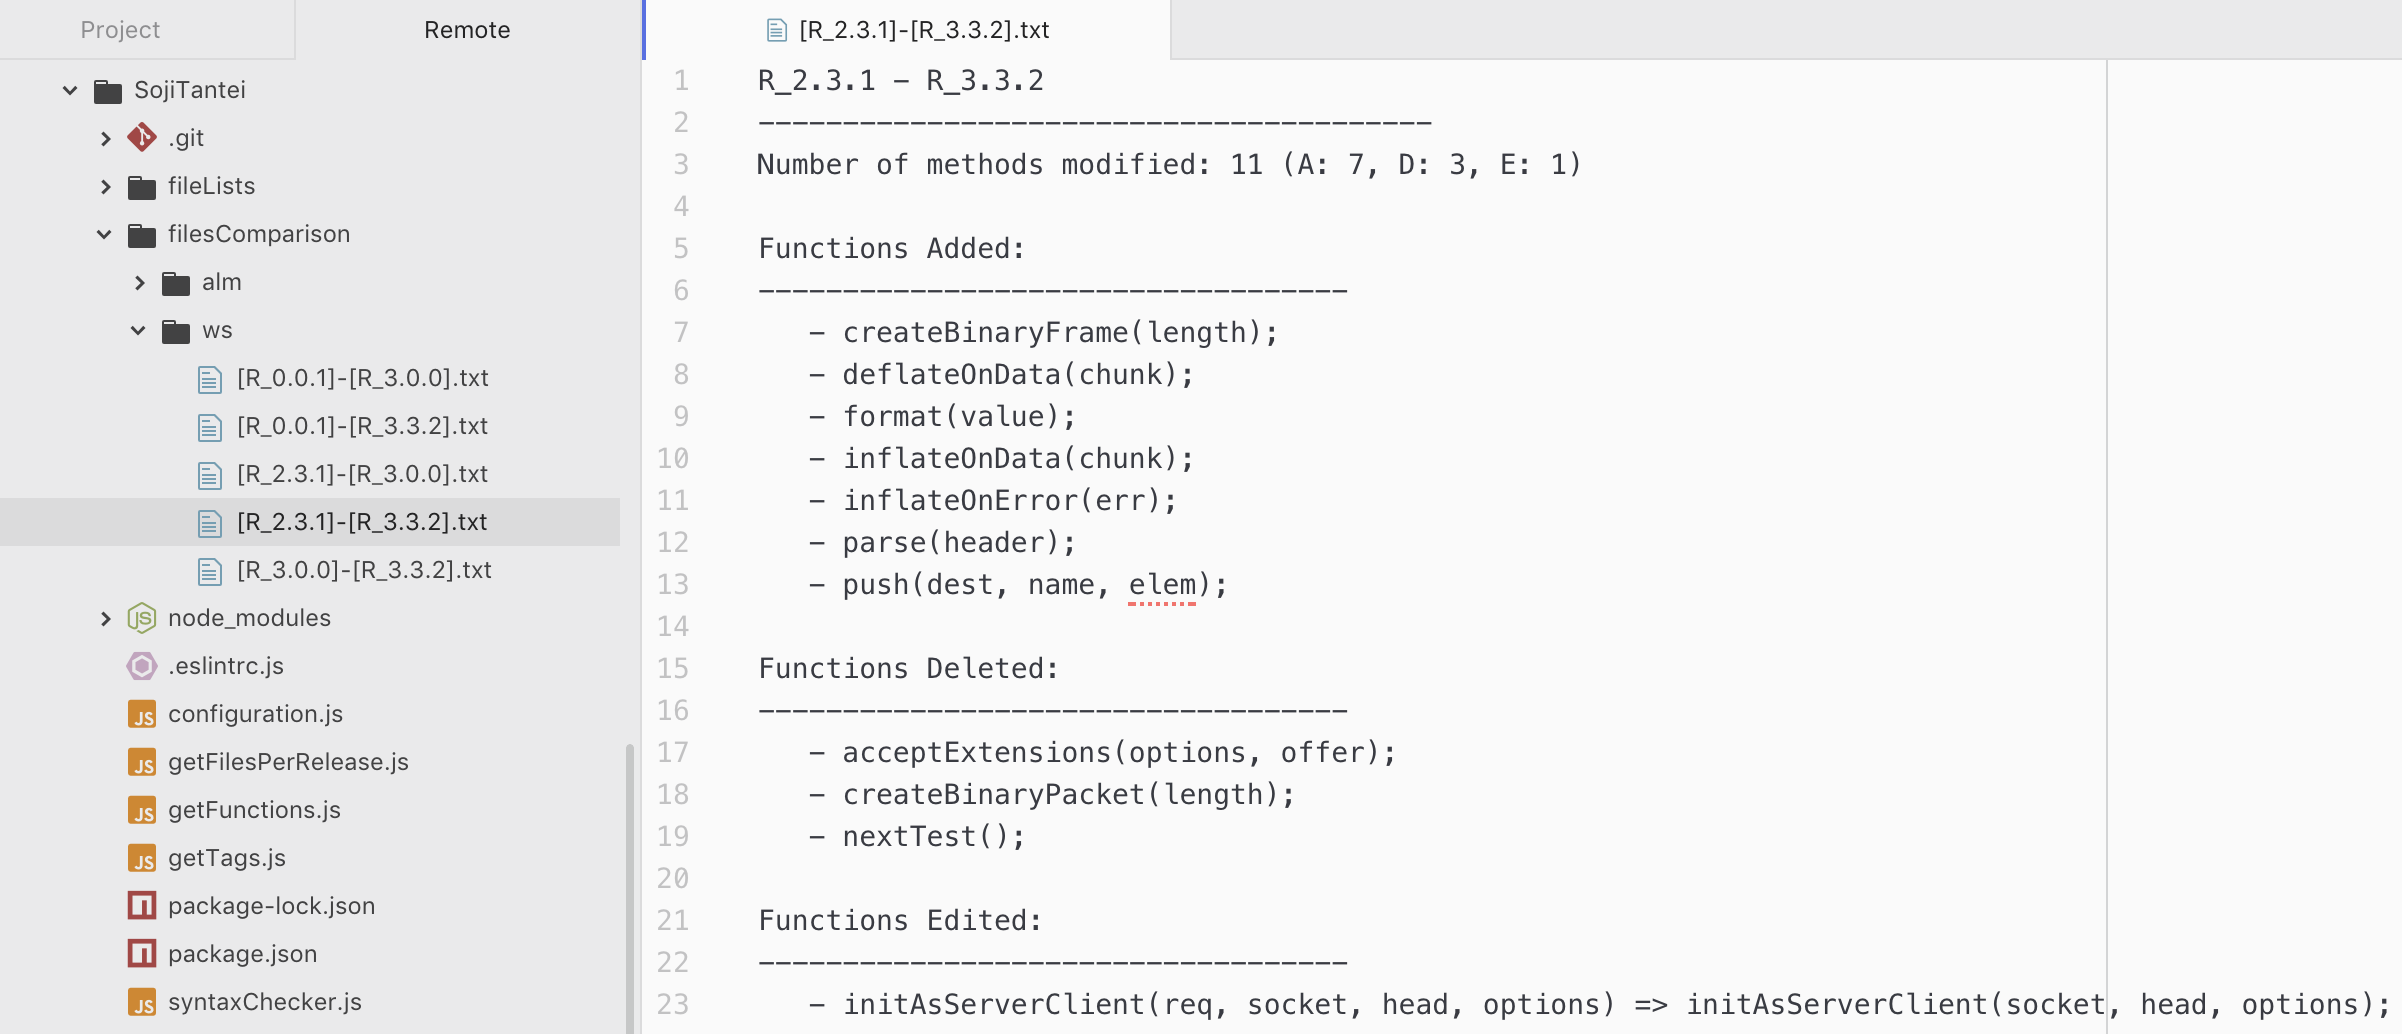
\includegraphics[width=1\textwidth]{images/comparison_example.png}
\caption{Example of the function comparison performed in versions 2.3.1 and 3.3.2 of \textit{ws} library}
\label{fig:compExample}
\end{figure}
%%%%%%%%%%%%%%%%%%%%%%%%%%%%%%%%%%%%% 

To execute this functionality the user need to execute the script called \textit{getFunctions.js} and input the name of the project to be analyzed in the first parameter.
There are two possible executions of the script,
(i) running the script without extra parameters will get the function comparison for all the version projects included in the output of Version Detector, this comparison will be performed by pairs in incremental order from the oldest version to the newest.
\enlargethispage{\baselineskip}
(ii) running the script inputting from the second parameter the names of version files (i.e. R\_\{version\}.txt) included in the output of Versions Detector will perform the analysis on those fails only, performed by pairs in the inputted order.\\

\tool[] is available for download by following the next url: \url{https://github.com/rodrigo-e/SojiTantei}.
The installation folder should contain all the scripts that are shown in Figure \ref{fig:sojiGit}

%%%%%%%%%%%%%%%%%%%%%%%%%%%%%%%%%%%%%
\begin{figure}[ht!]
\centering
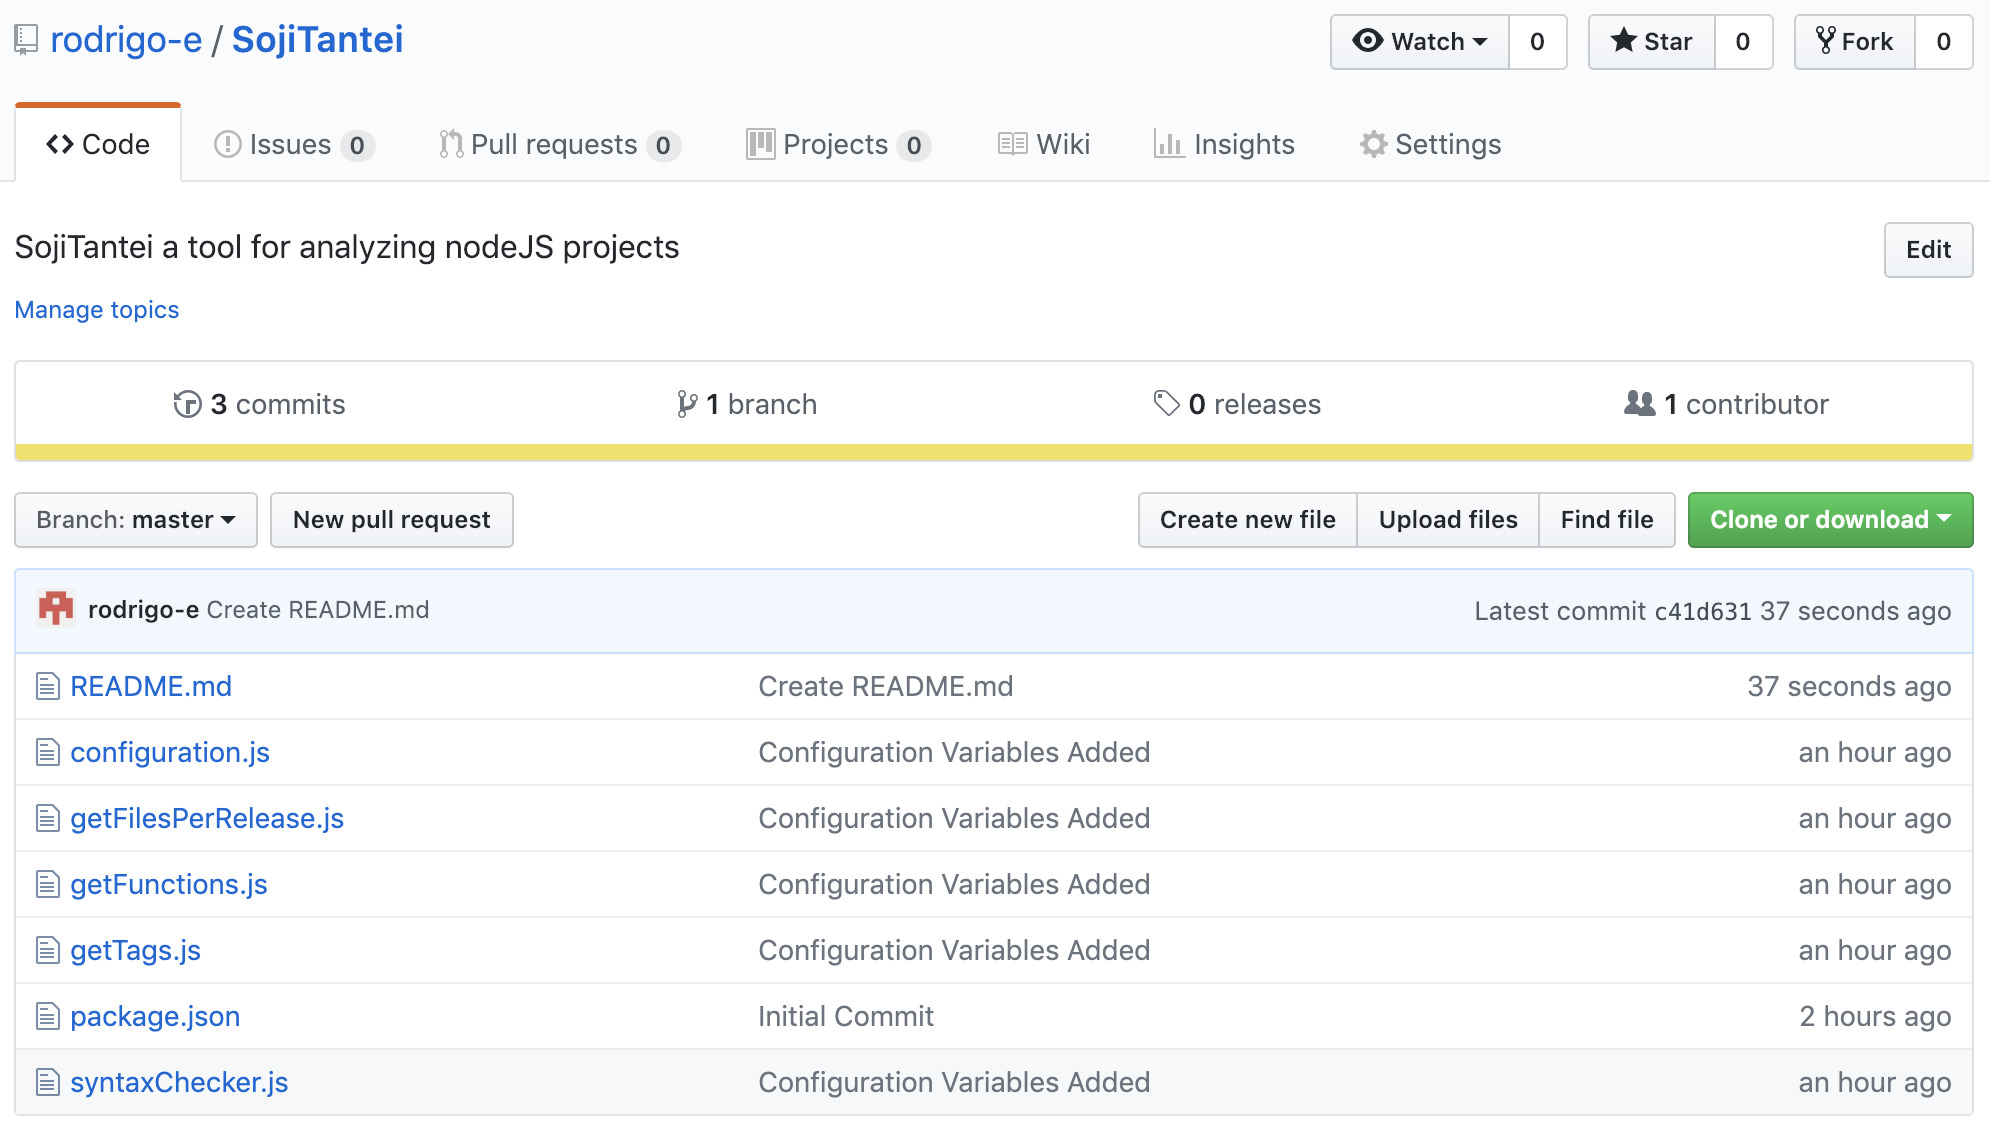
\includegraphics[width=1\textwidth]{images/soji_git.png}
\caption{Scripts of \tool[] in git repository}
\label{fig:sojiGit}
\end{figure}
%%%%%%%%%%%%%%%%%%%%%%%%%%%%%%%%%%%%%  

After downloading the tool you can follow the Readme file included to complete the installation.